%%%%% Document Setup %%%%%%%%

\documentclass[12pt, twocolumn]{revtex4}    % Font size (12pt) and column number (one or two).

\usepackage{times}                          % Times New Roman font type

\usepackage[a4paper, left=2.5cm, right=2.5cm,
 top=2.5cm, bottom=2.5cm]{geometry}       % Defines paper size and margin length

\renewcommand{\baselinestretch}{1.15}     % Defines the line spacing

\usepackage[font=small,
labelfont=bf]{caption}                      % Defines caption font size and caption title bolded

\usepackage{graphics,graphicx,epsfig,ulem}	% Makes sure all graphics works
\usepackage{amsmath}                        % Adds mathematical features for equations
\usepackage{float}

\usepackage{etoolbox}                       % Customise date to preferred format
\makeatletter
\patchcmd{\frontmatter@RRAP@format}{(}{}{}{}
\patchcmd{\frontmatter@RRAP@format}{)}{}{}{}
\renewcommand\Dated@name{}
\makeatother

\def\thesection{\arabic{section}}

\def\bibsection{\section*{References}}        % Position reference section correctly

%%%%% Document %%%%%
\begin{document}                     


\title{A Model for the Evolution of Quasars} 
\date{Submitted: \today{}}
\author{Joseph Carter}
\affiliation{\normalfont Level 4 Project, MPhys Physics with Astronomy\\ Supervisor: Professor T. Theuns\\ Department of Physics, Durham University}

\begin{abstract}              
 
Abstract abstract abstract abstract abstract abstract abstract abstract abstract abstract abstract abstract abstract abstract abstract abstract abstract abstract abstract abstract abstract abstract abstract abstract abstract abstract abstract abstract abstract abstract abstract abstract abstract abstract abstract abstract abstract abstract abstract abstract abstract abstract abstract abstract abstract abstract abstract abstract abstract abstract abstract abstract abstract abstract 

\end{abstract}


\maketitle
%\thispagestyle{plain} % produces page number for front page
\onecolumngrid


\tableofcontents
\newpage
\twocolumngrid
%%\let\toc@pre\relax
%%\let\toc@post\relax


\section{Introduction}

%%% example text follows %%%
Lorem ipsum dolor sit amet, consectetur adipiscing elit. Sed lacinia diam id odio consequat, vel cursus lectus aliquam. Quisque quis neque massa. Phasellus ut mi nulla. Morbi egestas urna mauris, sit amet accumsan nibh accumsan id. Etiam quis urna at felis imperdiet euismod non eget ligula. Vivamus sit amet ultricies massa.

\onecolumngrid


\begin{figure}[H]
\centering
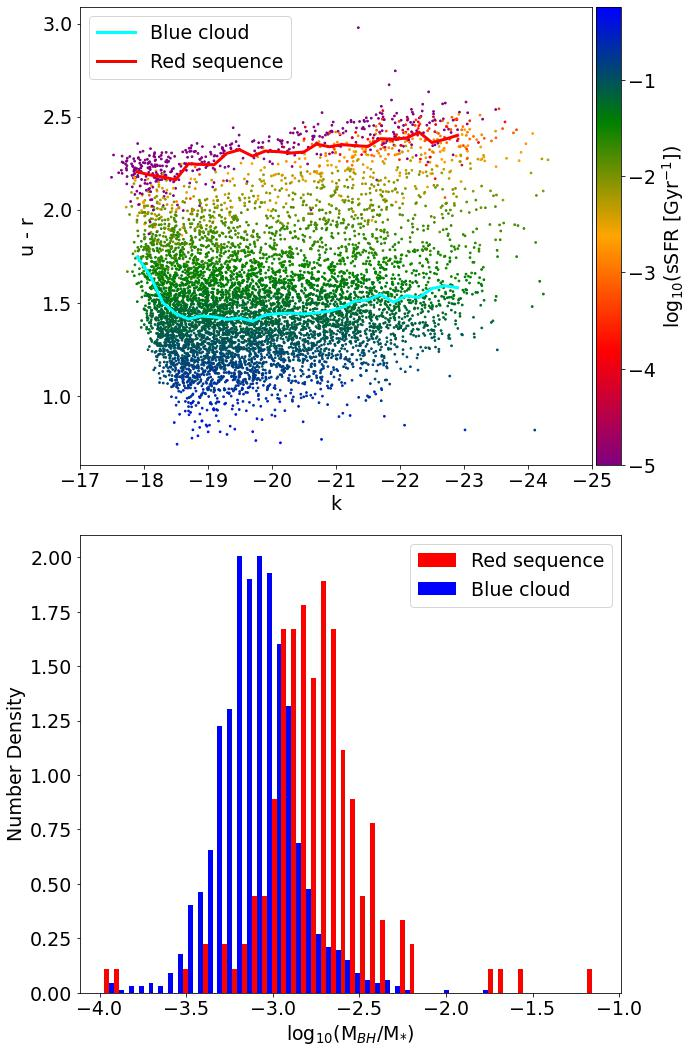
\includegraphics[width=11cm]{Plot_1.jpeg}
\caption{Top: u-r magnitude as a function of stellar mass for galaxies of mass greater than $10^9M_\odot$. Individual galaxies are plotted as points, coloured by sSFR, using the colourbar to the right. Middle: Histogram of sSFR for galaxies of stellar mass between $10^{10} - 10^{10.5}M_\odot$ (the shaded region on the above plot). Bottom: Histogram of $M_{BH}/M_*$ for galaxies of stellar mass between $10^{10} - 10^{10.5}M_\odot$.}
\label{fig:1}
\end{figure}
\twocolumngrid


\newpage

Random Latin text.

\onecolumngrid


\begin{figure}[H]
\centering
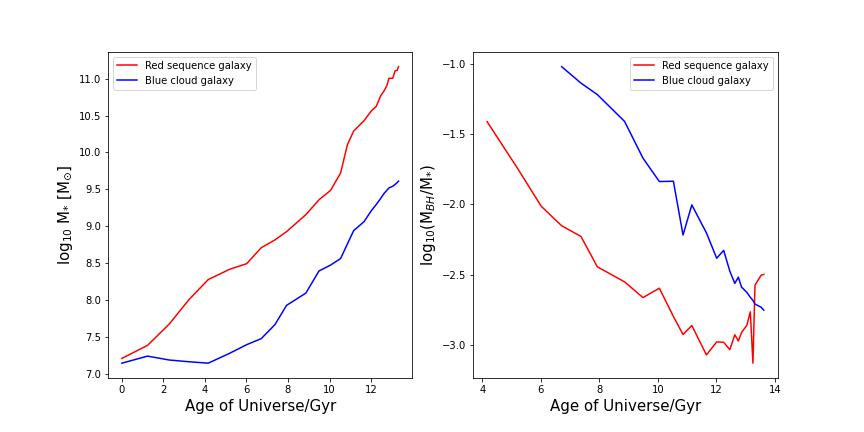
\includegraphics[width=14cm]{Plot_2.jpeg}
\caption{Plots of stellar mass, halo mass and black hole mass of two galaxies, one from the red sequence and one from the blue cloud, over cosmic time. The colour of the points show sSFR compared to the mean sSFR for central galaxies at that redshift. Colours from low to high sSFR: (cyan, blue, green, red, black).}
\label{fig:2}
\end{figure}
\twocolumngrid


\newpage

Random Latin text.

\onecolumngrid


\begin{figure}[H]
\centering
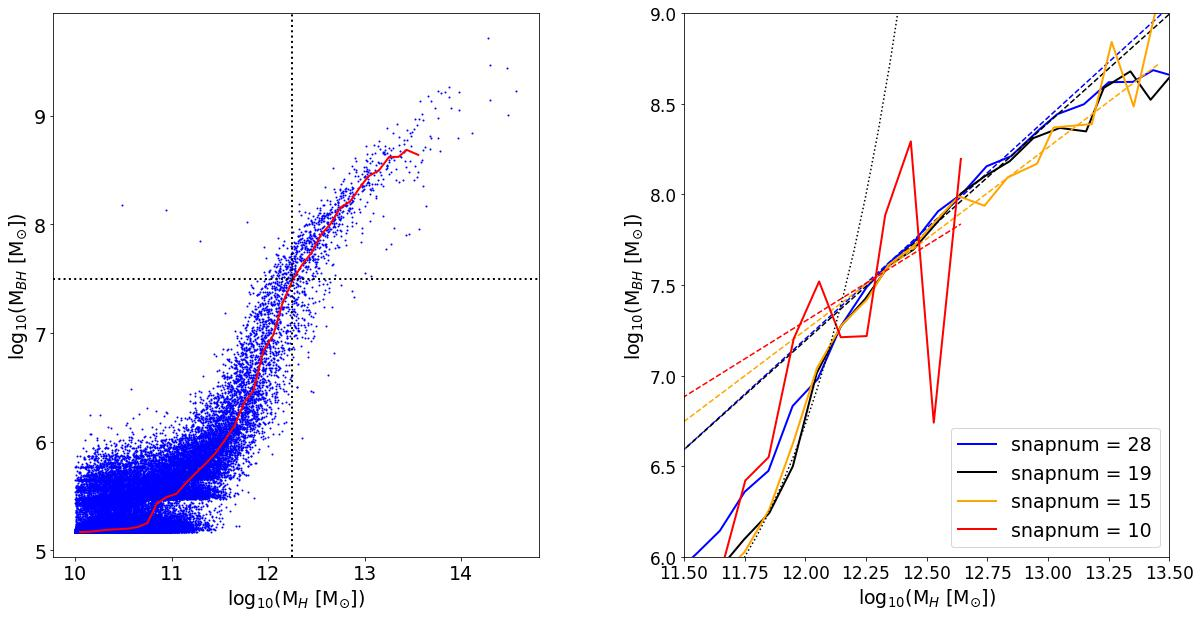
\includegraphics[width=17cm]{Plot_3.jpeg}
\caption{Left: Black hole mass - halo mass relation for central galaxies at z=0, the blue line shows median black hole mass. Right: Median black hole mass as a function of halo mass for central galaxies at z=0, z=1, z=2 and z=4. Dashed lines show power law fits, the dotted line shows an exponential fit.}
\label{fig:3}
\end{figure}
\twocolumngrid


Random Latin text.

\onecolumngrid


\begin{figure}[H]
\centering
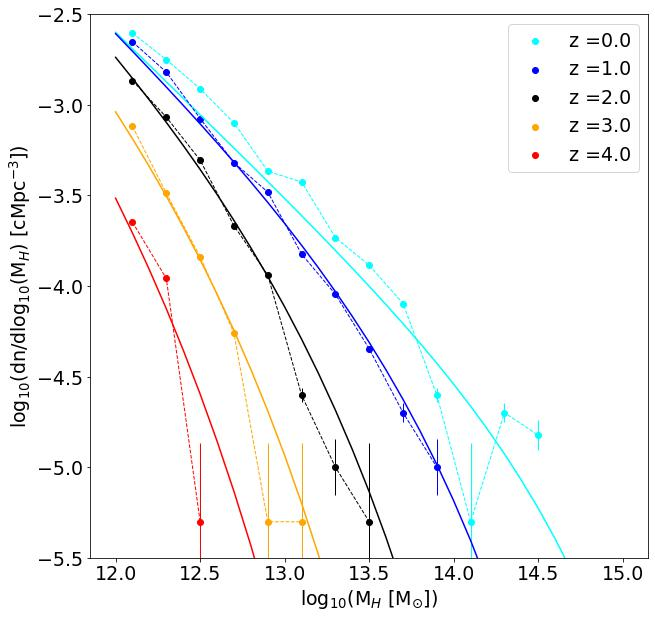
\includegraphics[width=\linewidth]{Mass_Function.jpeg}
\caption{Galaxy halo mass functions for galaxies of halo mass greater than $10^{12}M_\odot$ between z=0 and z=4. The filled lines show mass functions from EAGLE, dashed lines show mass functions from [Colossus].}
\label{fig:4}
\end{figure}
\twocolumngrid


Random Latin text.

\onecolumngrid


\begin{figure}[H]
\centering
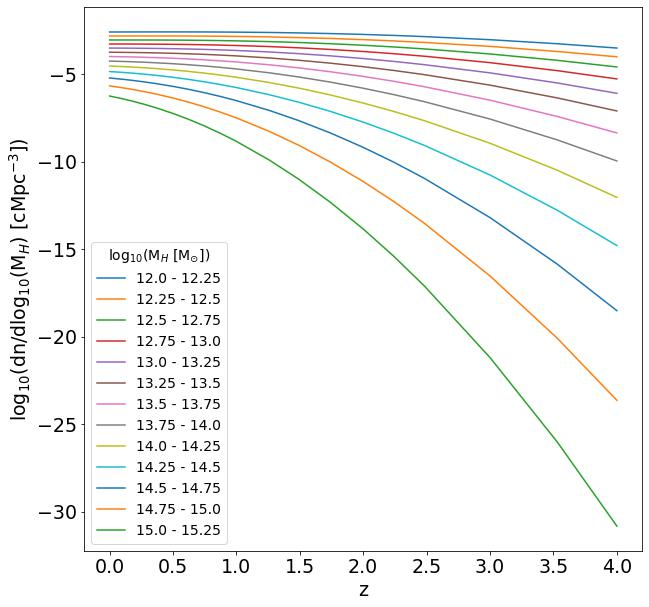
\includegraphics[width=\linewidth]{Mass_Function_2.jpeg}
\caption{Galaxy halo mass function as a function of redshift for galaxies of halo mass greater than $10^{11}M_\odot$.}
\label{fig:5}
\end{figure}
\twocolumngrid


\section{Section heading}

Duis eget tellus tortor. Cum sociis natoque penatibus et magnis dis parturient montes, nascetur ridiculus mus. In tellus nulla, sodales eu pulvinar at, accumsan quis magna. Nunc sed lacus diam. Nam enim mauris, imperdiet ut egestas quis, tincidunt at odio. Ut viverra nulla at libero dictum aliquet. Suspendisse lacus lacus, imperdiet nec elit nec, ullamcorper facilisis ex.

\subsection{Subsection heading}

Proin sit amet mauris tincidunt, consectetur nisi ultrices, dapibus elit. Nullam vitae faucibus odio, pharetra ultrices tortor. Class aptent taciti sociosqu ad litora torquent per conubia nostra, per inceptos himenaeos. 

\section{Conclusions}
Donec finibus, tellus sit amet luctus sodales, lectus ante accumsan ligula, at condimentum lorem justo a sapien. Phasellus vel tortor vitae metus lacinia efficitur ac vel ex. Aenean eget congue leo. Aliquam cursus mauris sit amet arcu dignissim, vel condimentum nisi sodales. 

\begin{acknowledgments}

(OPTIONAL) The author would like to thank...

\end{acknowledgments}

\begin{thebibliography}{}

bibitem{ref01} A.~N.~Other, Title of the book, edition, publishers, place of publication (year of publication), p.~123.   % example book reference 

bibitem{ref02} A.~N.~Other, Title of the article, journal title, volume, 123--456 (year of publication).   % example journal reference 

 You might prefer to use a different referencing style such as one where the references appear as "Smith et al. (1999)" with an alphabetical list at the end.

\end{thebibliography} 

\end{document}